\documentclass[a4paper,12pt]{article}
\usepackage[utf8]{inputenc}
\usepackage[english]{babel}
\usepackage{fancyhdr}
\usepackage{float}
\usepackage{hyperref}



%Use this to customize margins
\usepackage[
  top=2cm,
  bottom=2cm,
  left=1cm,
  right=1cm,
  headheight=17pt, % as per the warning by fancyhdr
  includehead,includefoot,
  heightrounded, % to avoid spurious underfull messages
]{geometry} 

%Use this to customize headers
\pagestyle{fancy}
\fancyhf{}
\fancyhead[LE,RO]{Report version: \today}
\fancyhead[RE,LO]{ReMeltRadar 2021/22}
\fancyfoot[CE,CO]{\leftmark}
\fancyfoot[LE,RO]{\thepage}
\usepackage{graphicx}
\renewcommand{\headrulewidth}{2pt}
\renewcommand{\footrulewidth}{1pt}


\usepackage{blindtext}

%Use this to customize tables
\usepackage[table]{xcolor}
\setlength{\arrayrulewidth}{1mm}
\setlength{\tabcolsep}{18pt}
\renewcommand{\arraystretch}{1.5}
%\arrayrulecolor[HTML]{fffff}

%Use this to customize colors
\definecolor{babyblueeyes}{rgb}{0.63, 0.79, 0.95}
\definecolor{beaublue}{rgb}{0.74, 0.83, 0.9}
\definecolor{bluegray}{rgb}{0.4, 0.6, 0.8}

%Here some pre-defined commands
\newcommand{\ProtocolTable}[6]
{
\begin{table}[]
\begin{tabular}{|p{1.8cm} p{3.8cm} p{1.8cm} p{2.0cm}|}
\hline
 \rowcolor{beaublue}\textbf{Name}:&\multicolumn{3}{l}{#1} Note \\
 \rowcolor{beaublue}\textbf{Folder:}&\multicolumn{3}{l}{#2} Note \\
 \rowcolor{beaublue}\textbf{Instrument:}&#3&\textbf{Date:}&#4 Note \\
  \rowcolor{beaublue}\textbf{Operator:}&#5&\textbf{Location:}&#6\\
\hline
\end{tabular}
\end{table}
}

%Start the document here.

\begin{document}
\section{Summary of ReMeltRadar 2021/22}
\textbf{RD}

\begin{figure}
  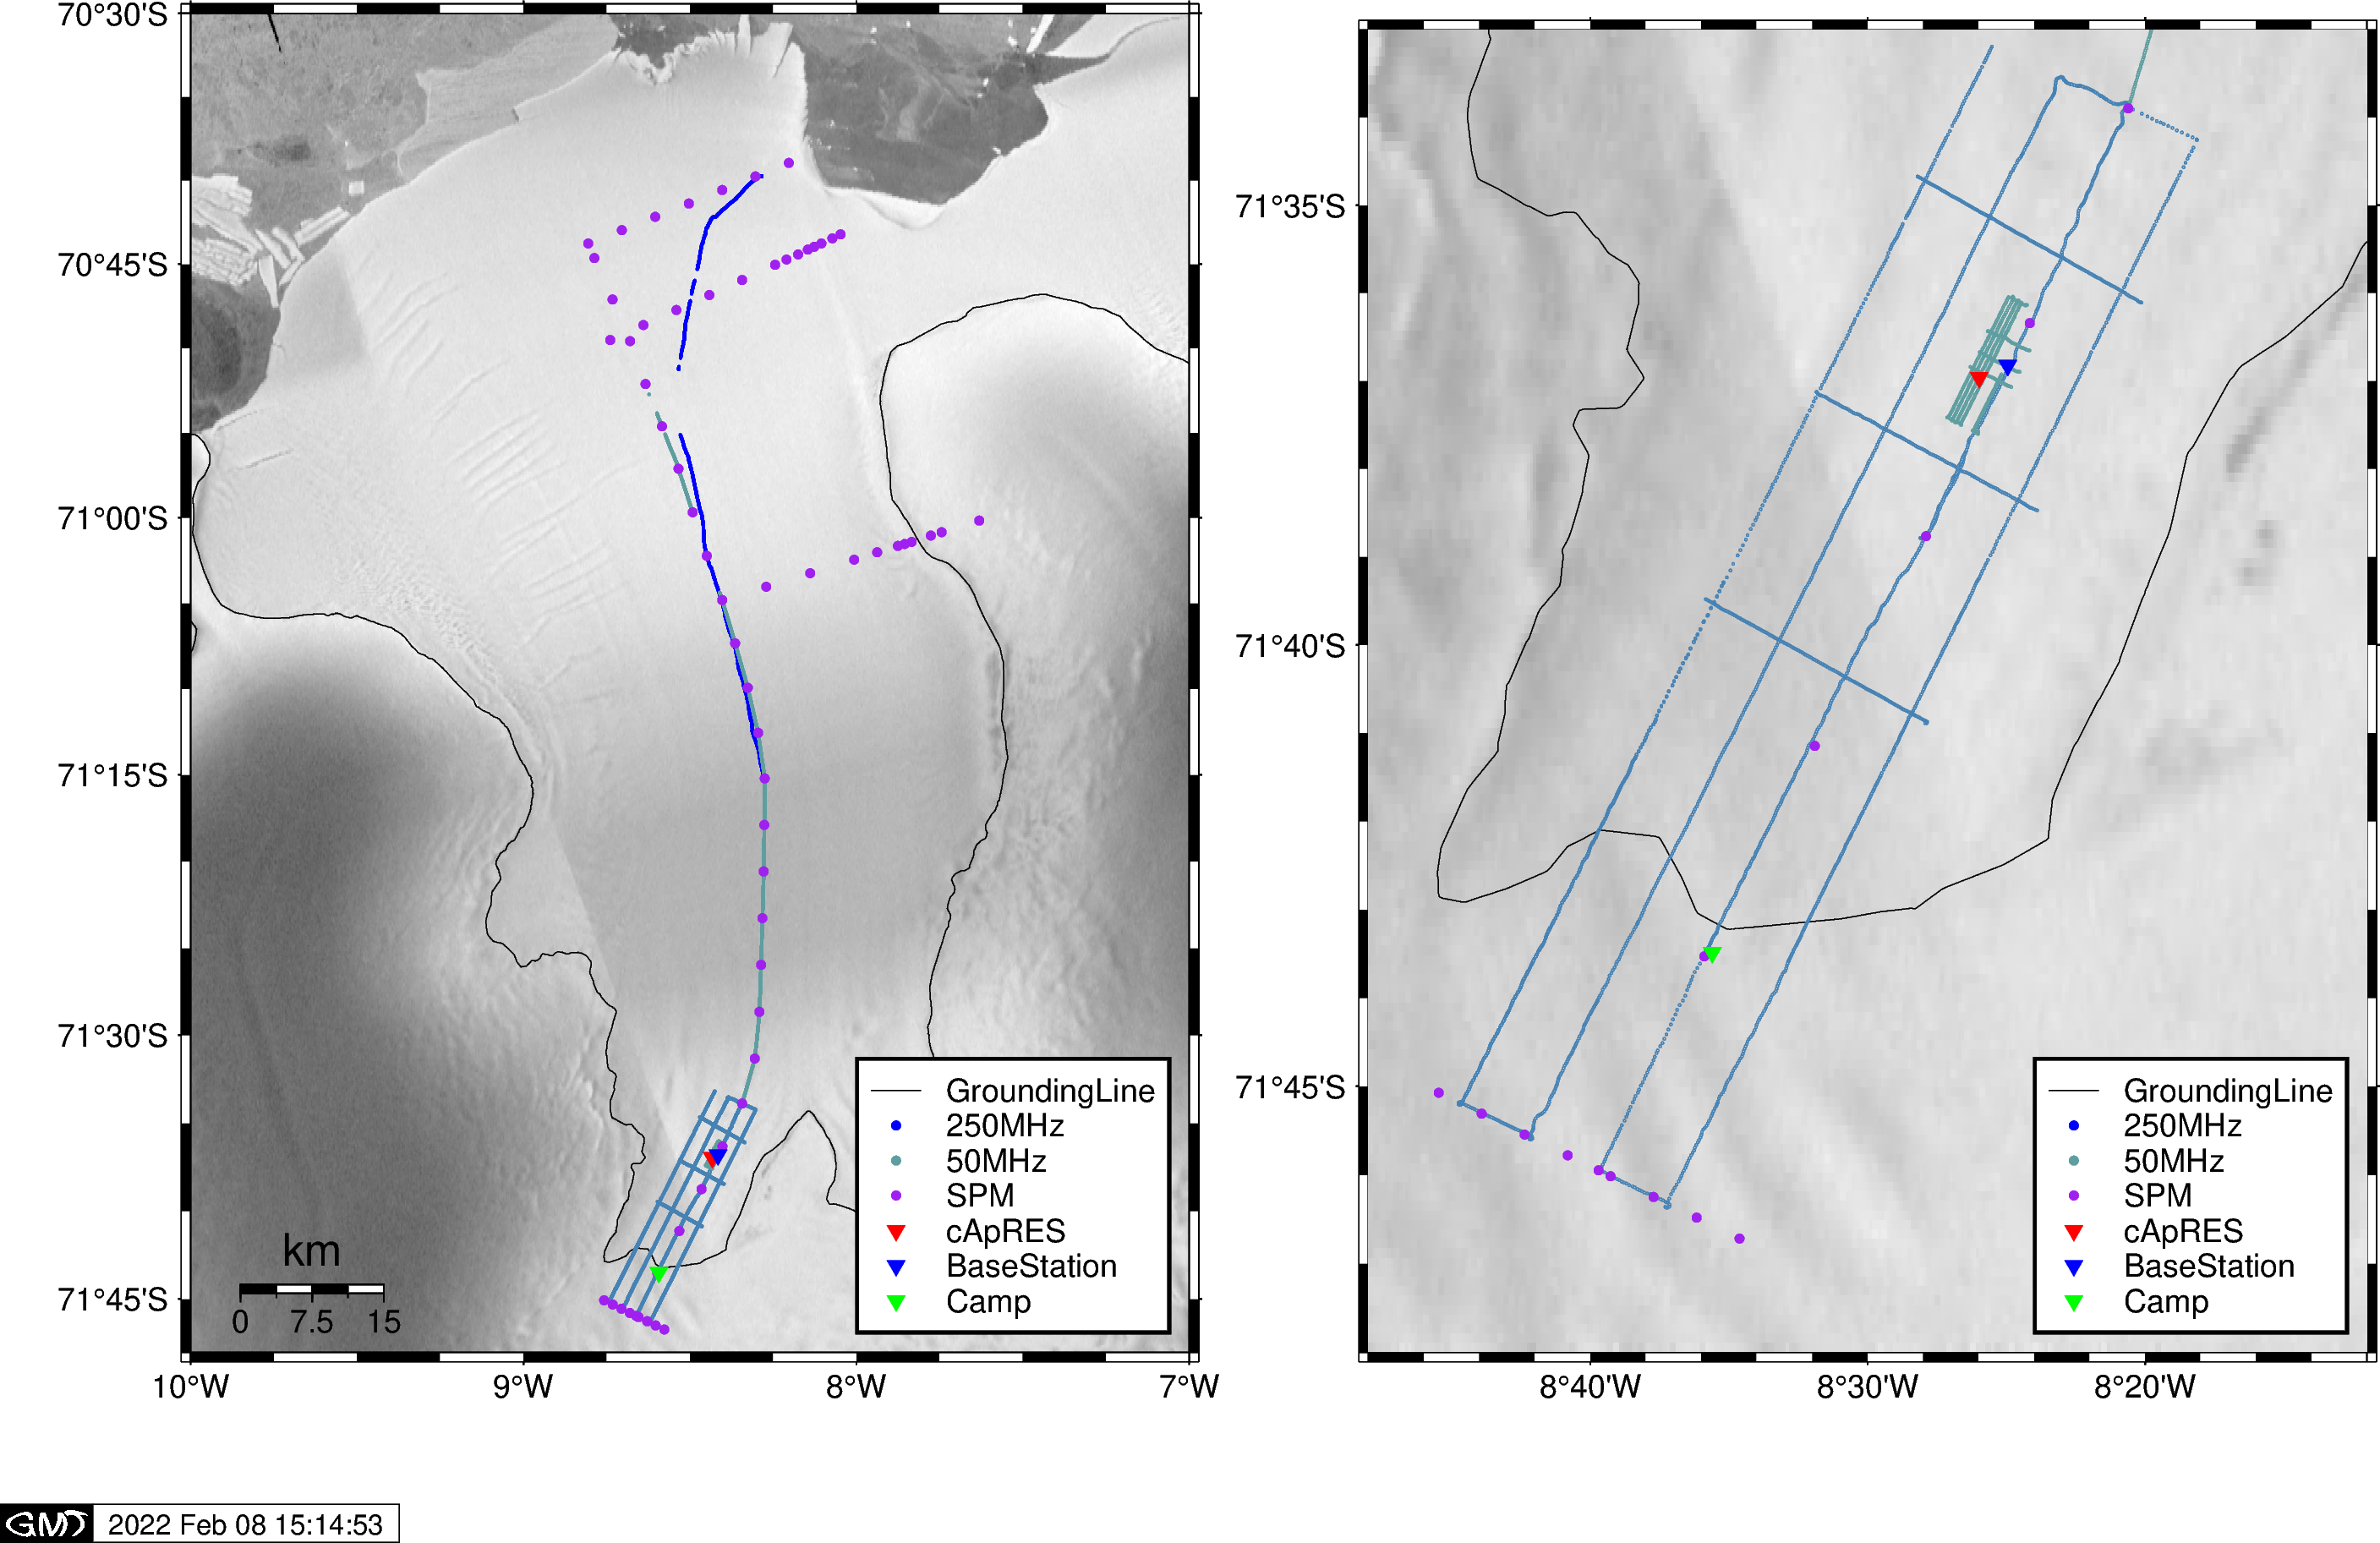
\includegraphics[width=\linewidth]{Figures/Overview.png}
  \caption{(Left) Larger-scale bird's eyes perspective of 250 MHz GPR, 50 MHz GPR, static \& polarimetric (SPM) and continuous ApRES (cApRES) locations at Ekström Ice Shelf, East Antarctica. (Right) Close-up of the survey grid close to the grounding-zone.}
  \label{fig:overview}
\end{figure}
ReMeltRadar's scientific focus (1) to understand \& quantify processes that
govern ocean-induced melting at the base of ice shelves, and (2) to provide
observational constraints on the spatial variability of ice rheology impacting
ice-shelf buttressing strength. The area of interest is the Ekström Ice Shelf,
East Antarctica, using the Neuyamer III station as a logistical hub for field
surveys on the ice shelf and in the grounding zone. The first field season took
place from November 2021 to January 2022. This report details the data collected
and will serve as a baseline for envisaged repeat measurements in 2022/23. 
%% ******************************************************
%% ******************************************************
\pagebreak
%% ******************************************************
%% ******************************************************
\subsection{Team composition and chronology of data collection}
\begin{table}
\rowcolors{2}{gray!25}{white}
\begin{tabular}{llll}
  \rowcolor{gray!50}
  Name & Project& Deployment& Responsibility\\
  \hline
  Inka Koch (UT) & ReMeltRadar & 27.12.21-13.12.22& PulseEkko GPR\\
  Jonathan Hawkins (UCL) & ReMeltRadar  &27.12.21-13.12.22& HF ApRES\\
  Reinhard Drews (UT) & ReMeltRadar  &27.12.21-13.12.22& Science Coordination\\
  Reza Ershadi (UT) & ReMeltRadar &05.11.21-13.12.22& Rover, SPM\\
  Olaf Eisen (AWI) & ReMeltRadar  &05.11.21-13.12.22& Traverse Leader\\
  \hline
\end{tabular}
\caption{\label{TableGPR}Team composition of ReMeltRadar with members of University of Tübingen (UT), University College London (UCL), and Alfred Wegener Institute (AWI).}
\end{table}
\begin{table}
  \rowcolors{2}{gray!25}{white}
  \begin{tabular}{m{1.5cm} m{2.25cm} m{7cm} m{3cm}}
    \rowcolor{gray!50}
    Date & Frequency & Profile & File-ID\\
    \hline
    28.12.21 & 50, 100 MHz & Test profiles near NM& \textit{PE files}\\
    29.12.21 & 100 MHz & MPA01-MPA03, SPX4-SPX2 near NM& \textit{PE files}\\
    01.01.22 & 250 MHz  & NM-SPMA25 during traverse& \textit{PE files}\\
    02.01.22 & 50 MHz & GZ profiling along flow (SPMA25-SPMA21-GLPE3n-GLPE4s)& \textit{PE files}\\
    03.01.22 & 50 MHz & GZ profiling along flow (GLPE4s-GLPE1s-GLPE2n transfer to SPMA25)& \textit{PE files}\\
    04.01.22 & 50 MHz & GZ profiling along flow (GLPE7n-GLPE8s-GLPE5s)& \textit{PE files}\\
    05.01.22 & 50 MHz & GZ profiling across flow (XX points XX)& \textit{PE files}\\
    06.01.22 & 50 MHz & Finegrid along flow (XX points XX)& \textit{PE files}\\
    09.01.22 & 50 MHz & Finegrid across flow (XX points XX)& \textit{PE files}\\
    10.01.22 & 50 MHz & Along-flow Camp-NM (SPMA21-SPMA10)& \textit{PE files}\\
    12.01.22 & 50 MHz & Camp-NM continuation (SPMA10 - XX)& \textit{PE files}\\
    \hline
  \end{tabular}
  \caption{\label{TableGPR}Overview of GPR measurements taken with the PulseEkko radar from Sensors\&Software. Details for the system setup and individual profiles are found in Section \ref{SecGpr}. Operator: I. Koch.}
Here we need a table such as table \label{TableGPR} for each sensor. 
\end{table}
%% ******************************************************
%% ******************************************************
\pagebreak
%% ******************************************************
%% ******************************************************
\section{Data structure and initial source codes}
\textbf{RD, JH}
%% ******************************************************
%% ******************************************************
\pagebreak
%% ******************************************************
%% ******************************************************
\section{GPR: Data example, field picture, system setup and profile specifics}
\label{SecGpr}
\textbf{IK}
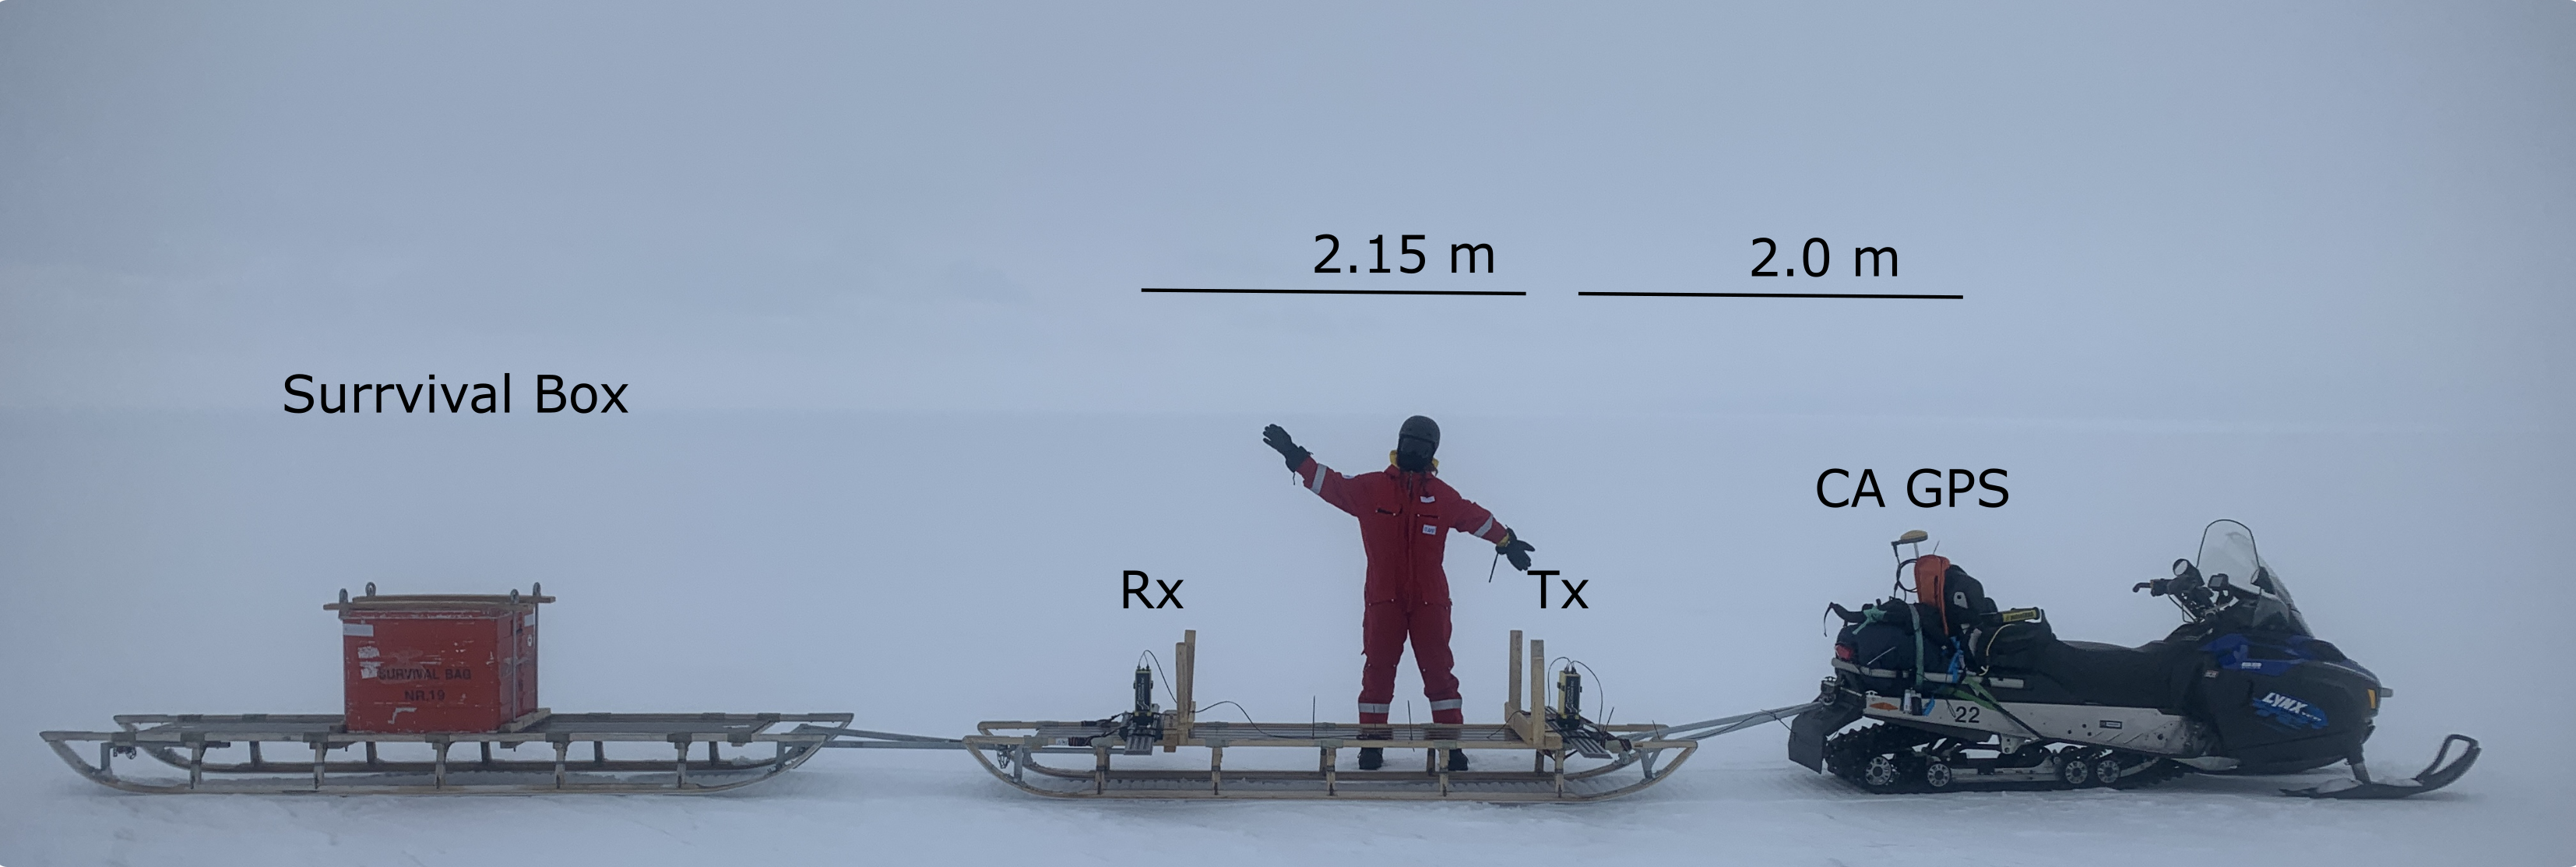
\includegraphics[width=\textwidth]{Figures/PulseEkko/RadarSetup.png}
%% ******************************************************
%% ******************************************************
\pagebreak
%% ******************************************************
%% ******************************************************
\section{SPM: Data example, field picture, system setup and site specifics}
\label{SecSPM}
\textbf{This section is written by Reza Ershadi}
(\href{mailto:mohammadreza.ershadi@uni-tuebingen.de}{\color{blue}{Email Me}})\\

The SPM points were measured in two different ways.
\begin{itemize}
\item We drove to the point by
Hilux. We set up the system (ApRES and antenna) every time at each point. In
this method, the antennas were directly on the snow surface (fig. \ref{fig_SPM_surface}). The
coordinates and date of the measurements are written in table (\ref{Table_SPM_surface}).
\item We fixed the system (ApRES and antenna) inside the sleds and drove to the points by a
snowmachine (fig. \ref{fig_SPM_sled}). The coordinates and date of the measurements are written in
table (\ref{Table_SPM_sled}).
\end{itemize}
More information on these points is in the following path:\\
..\textbackslash Tex\textbackslash Info\textbackslash RE\_SPM\_Points\_Info.csv\\
..\textbackslash Tex\textbackslash Info\textbackslash RE\_BulletPointReport.txt

\subsection{SPM: Antenna directly on snow surface}
\begin{figure}[H]
	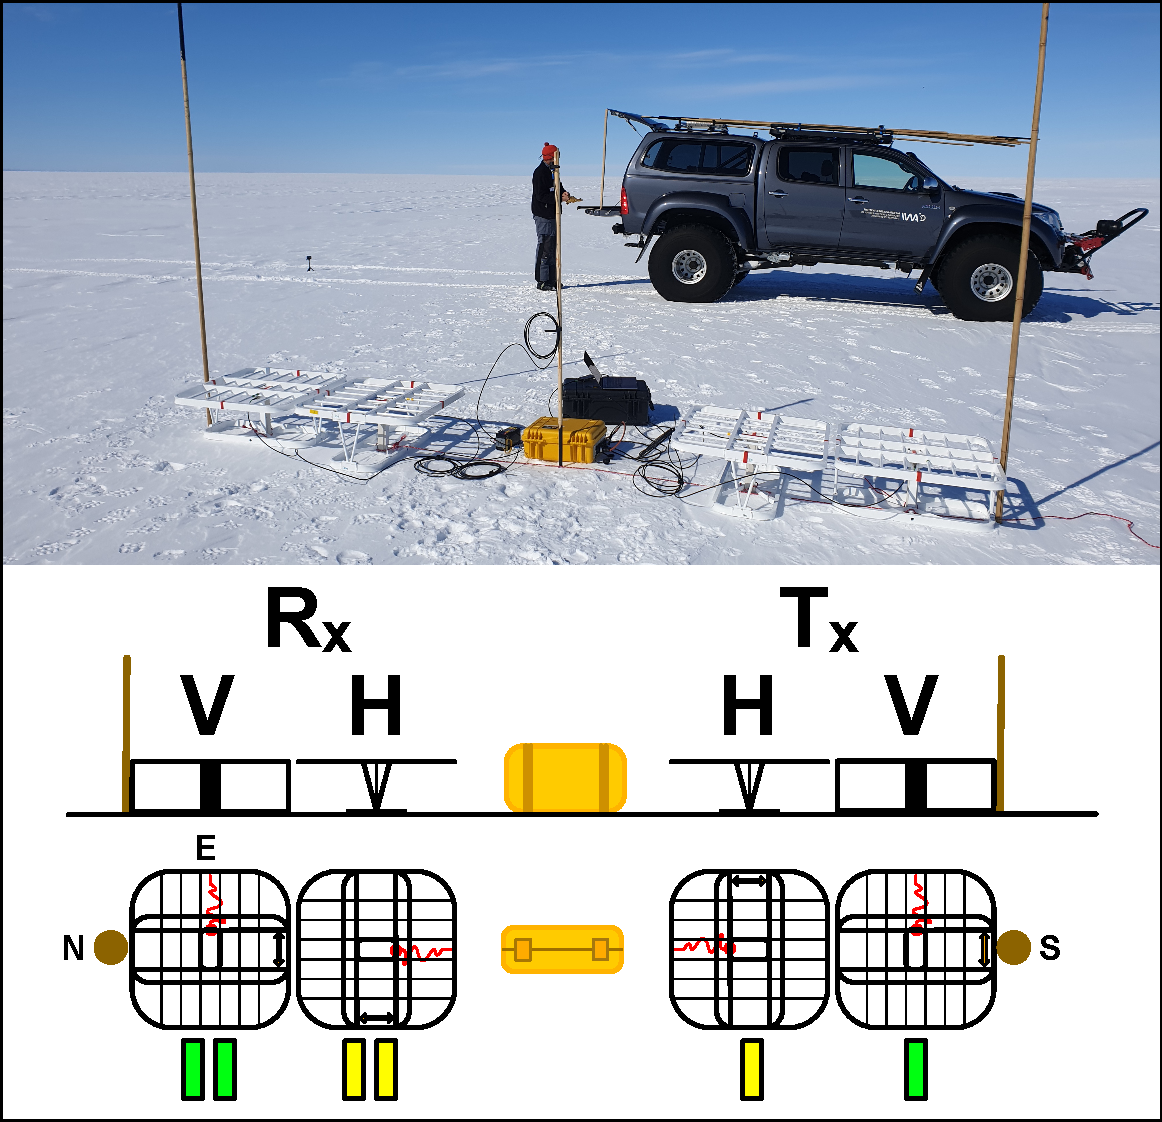
\includegraphics[width=\linewidth]{Figures/SPM_OnSurface.pdf}
	\caption{SPM four antenna (mimo) measurements. Antenna directly on the snow surface.
  The yellow and green rectangles are the tape sign an each antenna. 
  The brown sticks and circles are the bamboo poles.
  The system was positioned in a way that T was always in the South direction.}
	\label{fig_SPM_surface}
\end{figure}

\begin{table}[H]
  \tiny
  \centering
  \rowcolors{2}{gray!25}{white}
  \begin{tabular}[width=\textwidth]{c c c c c c}
    \rowcolor{gray!50}
    Name & Date & Latitude & Longitude & pRES & Note\\
    \hline
    SPM X 04 & 06.12.2021 &  &  & 127 & Unattened mimo test with RTK GPS running \\ 
    SPM A 01 & 06.12.2021 &  &  & 127 & Note \\
    SPM A 04 & 06.12.2021 &  &  & 127 & Note \\
    SPM A 06 & 07.12.2021 & S70 54.6083 & W8 35.0011 & 127 & Note \\
    SPM A 08 & 07.12.2021 & S70 59.6685 & W8 29.5190 & 127 & Note \\
    SPM A 10 & 07.12.2021 & S71 04.8188 & W8 24.1606 & 127 & Note \\
    SPM A 12 & 07.12.2021 & S71 09.9336 & W8 19.5682 & 127 & Note \\
    SPM A 11 & 07.12.2021 & S71 07.3516 & W8 21.8561 & 127 & Note \\
    SPM A 09 & 07.12.2021 & S71 02.2326 & W8 26.9498 & 127 & Note \\
    SPM A 07 & 07.12.2021 & S70 57.1200 & W8 32.0608 & 127 & Note \\
    SPM A 05 & 07.12.2021 & S70 52.1103 & W8 38.0142 & 127 & Note \\
    SPM X 12 & 07.12.2021 & S70 48.5407 & W8 37.3807 & 127 & Note \\
    SPM X 05 & 08.12.2021 & S70 42.1876 & W8 36.2362 & 127 & Note \\
    SPM X 06 & 08.12.2021 & S70 42.9845 & W8 42.2801 & 127 & Note \\
    SPM A 02 & 08.12.2021 & S70 44.6456 & W8 47.2300 & 127 & Note \\
    SPM A 03 & 08.12.2021 & S70 4?.0996 & W8 43.9270 & 127 & Note \\
    SPM X2 13 & 08.12.2021 & S70 49.5042 & W8 44.3598 & 127 & Note \\
    SPM X2 12 & 08.12.2021 & S70 48.6233 & W8 38.4010 & 127 & Note \\
    SPM X3 01 & 01.01.2022 & S71 0.1622 & W7 37.8862 & 127 & Note \\
    SPM X3 02 & 01.01.2022 & S71 0.8448 & W7 44.6390 & 127 & Note \\
    SPM X3 03 & 01.01.2022 & S71 1.0425 & W7 46.5675 & 127 & Note \\
    SPM X3 04 & 01.01.2022 & S71 1.4077 & W7 50.0373 & 127 & Note \\
    SPM X3 05 & 01.01.2022 & S71 1.5366 & W7 52.3067 & 127 & Note \\
    SPM X3 06 & 01.01.2022 & S71 1.6515 & W7 52.5199 & 127 & Note \\
    SPM X3 07 & 01.01.2022 & S71 2.0236 & W7 56.2648 & 127 & Note \\
    SPM X3 08 & 01.01.2022 & S71 2.4512 & W8 0.4169 & 127 & Note \\
    SPM X3 09 & 01.01.2022 & S71 8.2488 & W8 8.3205 & 127 & Note \\
    SPM X3 10 & 01.01.2022 & S71 4.0086 & W8 16.2397 & 127 & Note \\
    SPM A 13 & 01.01.2022 & S71 12.5541 & W8 17.6910 & 127 & Note \\
    SPM A 14 & 01.01.2022 & S71 15.2070 & W8 16.5035 & 127 & Note \\
    SPM A 15 & 01.01.2022 & S71 17.8907 & W8 16.5801 & 127 & Note \\
    SPM A 16 & 01.01.2022 & S71 20.5795 & W8 16.6960 & 127 & Note \\
    SPM A 17 & 01.01.2022 & S71 23.2723 & W8 16.9177 & 127 & Note \\
    SPM A 18 & 01.01.2022 & S71 25.9609 & W8 17.1657 & 127 & Note \\
    SPM A 25 & 04.01.2022 & S71 43.5428 & W8 35.8674 & 128 & Note \\
    \hline
  \end{tabular}
  \caption{SPM on surface info}
  \label{Table_SPM_surface}
\end{table}

\begin{figure}[H]
	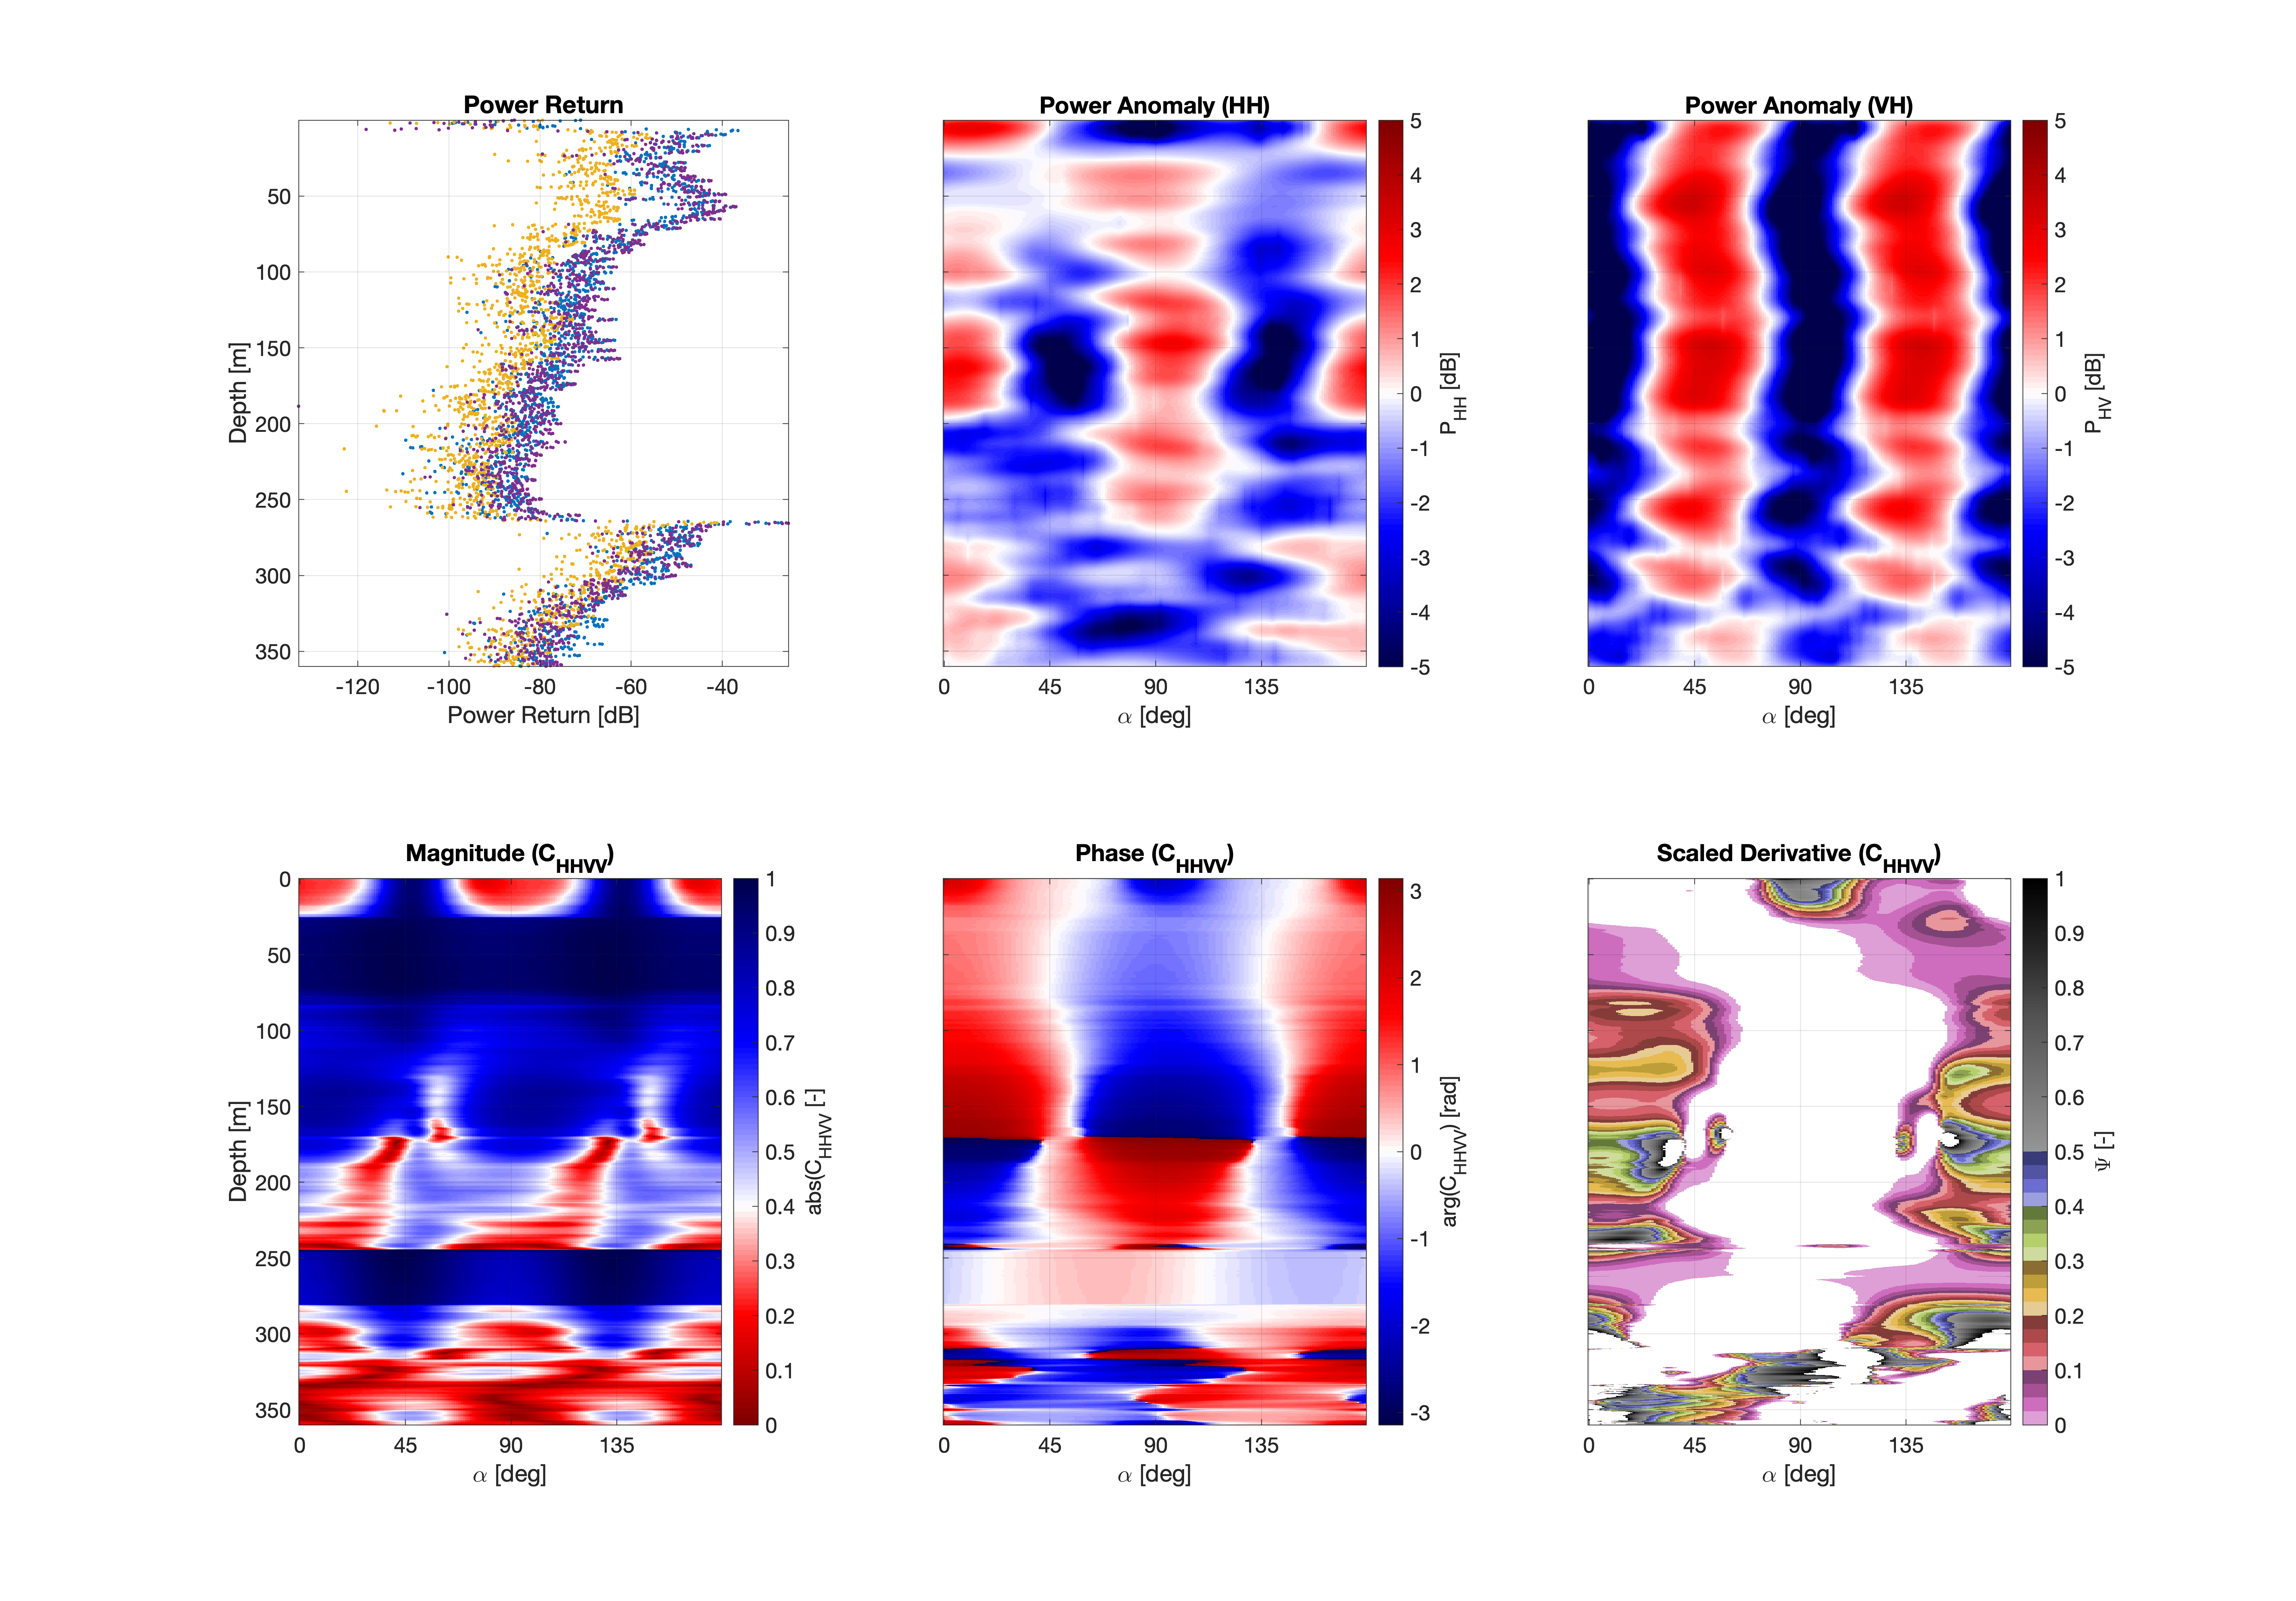
\includegraphics[width=\linewidth]{Figures/SPM_X_05.png}
	\caption{Data example from SPM\_X\_05 (floating ice - far from the GZ)}
	\label{fig_SPM_X_05}
\end{figure}

\begin{figure}[H]
	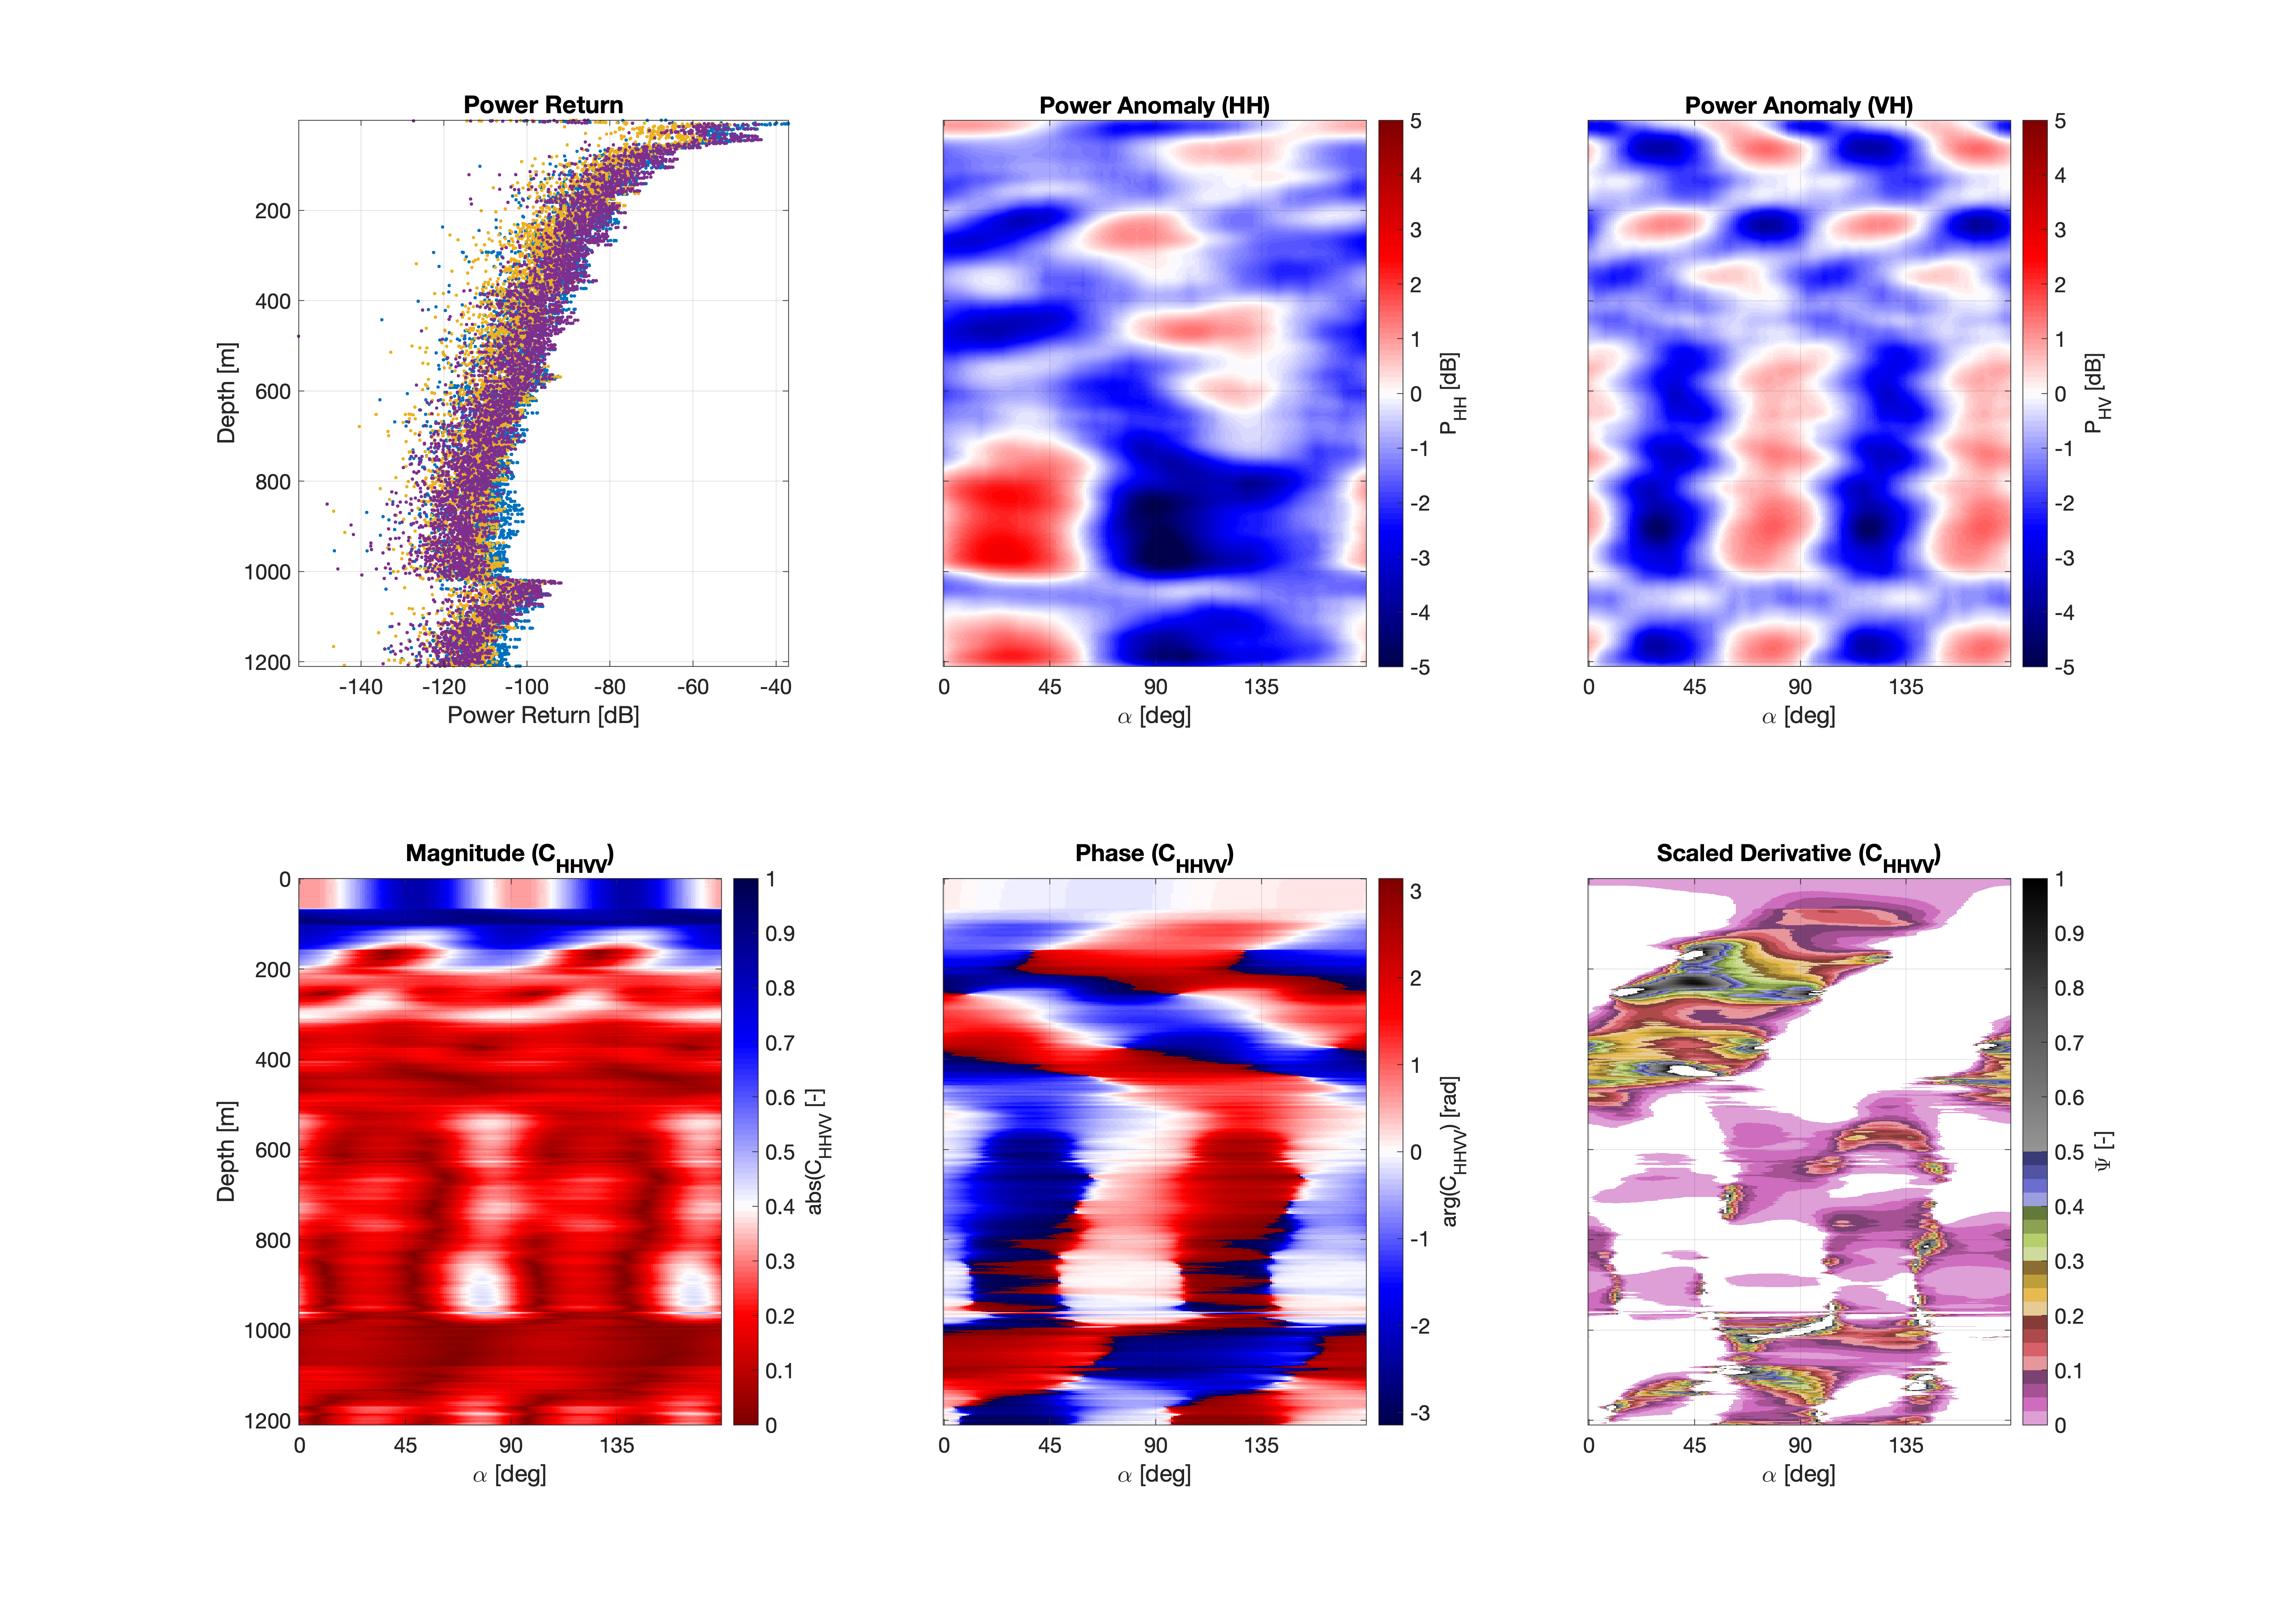
\includegraphics[width=\linewidth]{Figures/SPM_A_25.png}
	\caption{Data example from SPM\_A\_25 (grounded ice - very close to the GZ)}
	\label{fig_SPM_A_25}
\end{figure}

\subsection{SPM: Antenna inside the sleds}
\begin{figure}[H]
	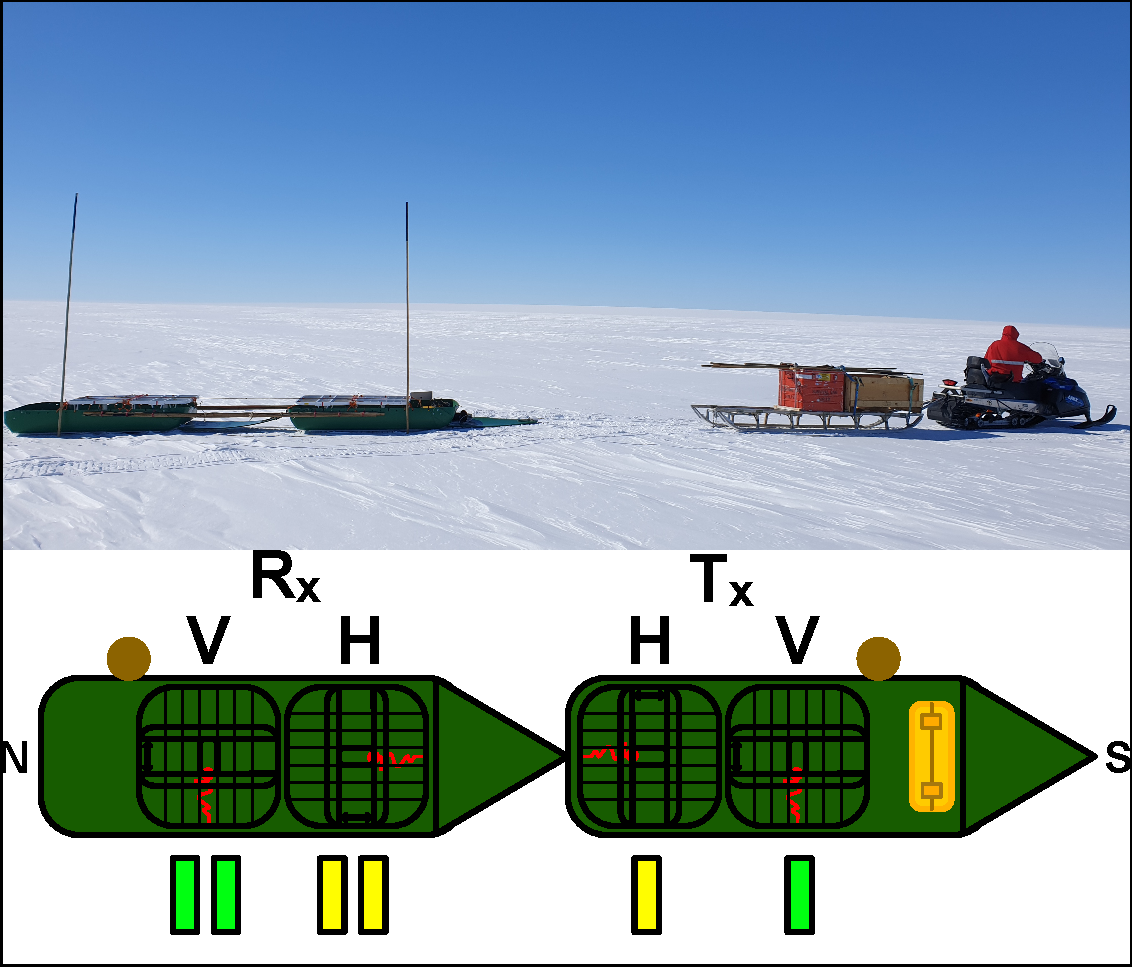
\includegraphics[width=\linewidth]{Figures/SPM_OnSled.pdf}
	\caption{SPM four antenna (mimo) measurements. Antenna inside sleds.
  The yellow and green rectangles are the tape sign an each antenna. 
  The brown sticks and circles are the bamboo poles. 
  The system was positioned in a way that T was always in the South direction.}
	\label{fig_SPM_sled}
\end{figure}

\begin{table}[H]
  \tiny
  \centering
  \rowcolors{2}{gray!25}{white}
  \begin{tabular}[width=\textwidth]{c c c c c c}
    \rowcolor{gray!50}
    Name & Date & Latitude & Longitude & pRES & Note\\
    \hline
    SPM X 01 & 10.12.2021 & S70 38.9781 & W8 12.1931 & 127 &  \\
    SPM X2 11 & 11.12.2021 & S70 47.7299 & W8 32.4452 & 127 &  \\
    SPM X2 10 & 11.12.2021 & S70 46.8444 & W8 26.5088 & 127 &  \\
    SPM X2 09 & 11.12.2021 & S70 45.9602 & W8 20.4776 & 127 &  \\
    SPM X 03 & 12.12.2021 & S70 40.5602 & W8 24.2193 & 127 &  \\
    SPM X 02 & 12.12.2021 & S70 39.7987 & W8 17.4478 & 127 &  \\
    SPM X2 01 & 13.12.2021 & S70 43.2433 & W8 2.8528 & ? &  \\
    SPM X2 02 & 13.12.2021 & S70 43.5002 & W8 4.3377 & ? &  \\ 
    SPM X2 03 & 13.12.2021 & ? & ? & ? & double check needed \\
    SPM X2 04 & 13.12.2021 & ? & ? & ? & double check needed \\
    SPM X2 05 & 13.12.2021 & S70 44.145 & W8 8.7386 & ? &  \\
    SPM X2 06 & 13.12.2021 & S70 44.4317 & W8 10.4649 & ? &  \\
    SPM X2 07 & 13.12.2021 & S70 44.7319 & W8 12.5599 & ? &  \\
    SPM X2 08 & 13.12.2021 & S70 45.0474 & W8 14.6026 & ? &  \\
    SPM A 22 & 7.01.2022 & S71 36.3400 & W8 24.1557 & 127 & Same setup as rover in traverse\\
    SPM A 19 & 7.01.2022 & S71 28.6556 & W8 17.4667 & 127 & Same setup as rover in traverse\\
    SPM A 20 & 7.01.2022 & S71 31.3291 & W8 18.3103 & 127 & Same setup as rover in traverse\\
    SPM A 21 & 7.01.2022 & S71 33.8910 & W8 20.5898 & 127 & Same setup as rover in traverse\\
    SPM A 23 & 7.01.2022 & S71 38.7621 & W8 27.8876 & 127 & Same setup as rover in traverse\\
    SPM A 24 & 7.01.2022 & S71 41.1405 & W8 31.9045 & 127 & Same setup as rover in traverse\\
    SPM X4 01 & 08.01.2022 & S71 25.0643 & W8 45.4317 & 127 & Same setup as rover in traverse\\
    SPM X4 02 & 08.01.2022 & S71 54.3048 & W8 43.9249 & 127 & Same setup as rover in traverse\\
    SPM X4 03 & 08.01.2022 & S71 45.5403 & W8 42.3649 & 127 & Same setup as rover in traverse\\
    SPM X4 04 & 08.01.2022 & S71 45.7?64 & W8 40.8149 & 127 & Same setup as rover in traverse\\
    SPM X4 05 & 08.01.2022 & S71 46.0135 & W8 39.2839 & 127 & Same setup as rover in traverse\\
    SPM X4 06 & 08.01.2022 & S71 46.2455 & W8 37.7977 & 127 & Same setup as rover in traverse\\
    SPM X4 07 & 08.01.2022 & S71 46.4827 & W8 36.1669 & 127 & Same setup as rover in traverse\\
    SPM X4 08 & 08.01.2022 & S71 46.7199 & W8 34.6045 & 127 & Same setup as rover in traverse\\
    \hline
  \end{tabular}
  \caption{SPM on sled info}
  \label{Table_SPM_sled}
\end{table}
%% ******************************************************
%% ******************************************************
\pagebreak
%% ******************************************************
%% ******************************************************
\section{MP\_A (profiling)}
\textbf{This section is written by Reza Ershadi}
(\href{mailto:mohammadreza.ershadi@uni-tuebingen.de}{\color{blue}{Email Me}})\\

The purpose here was to measure a 1000 m profile with 1.5 m spacing with all the
antennas positioned in the H direction. The system was directly connected to an
RTK GPS for precise positioning. We had many problems with this profile,
including the RTK signal, constant ApRES disconnection and typical rover
problems. Therefore, we could not finish the 1000 m profile with 1.5 m spacing.
The position of the profile and measured points are stored in our log files.\\

\textcolor{red}{Add detailed information about the 3 metal pieces. (?)}\\

The MP\_A profile has been done with two different methods.
\begin{itemize}
  \item We pulled the whole sled system manually for 100 m with 1.5 m spacing (fig. \ref{fig_MPA_manual}).
  \item We connected the sled system to the rover for a 1000 m profiling with 1.5 m spacing (fig. \ref{fig_MPA_rover})
\end{itemize}

\subsection{Manually pulling the sleds}
\begin{figure}[H]
	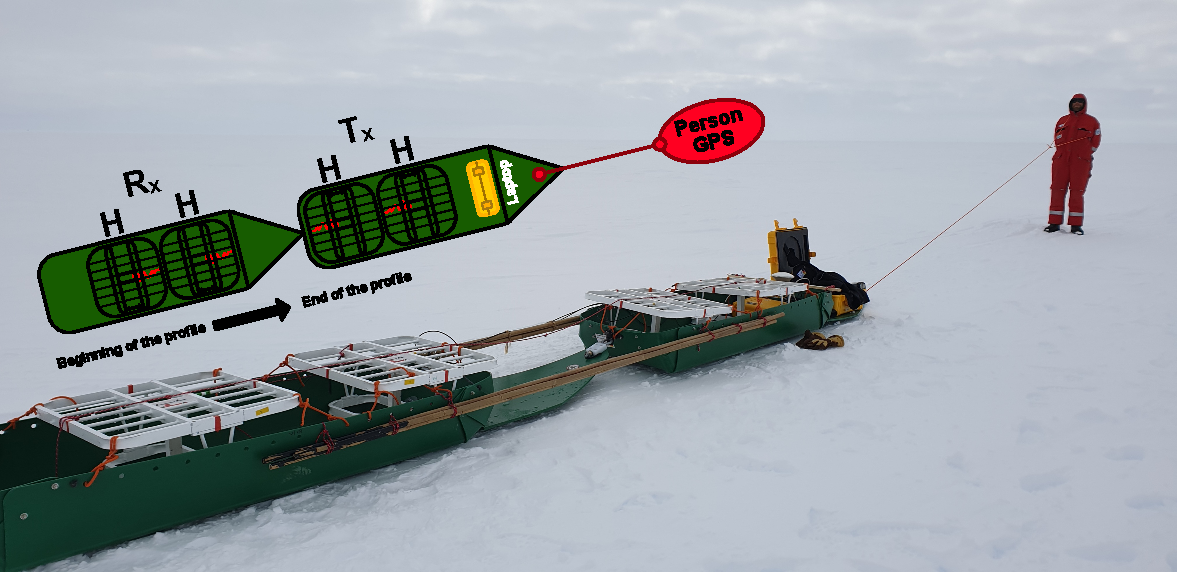
\includegraphics[width=\linewidth]{Figures/MPA_manual.pdf}
	\caption{Manually pulling the ApRES and sleds}
	\label{fig_MPA_manual}
\end{figure}

\subsection{Using the rover}
\begin{figure}[H]
	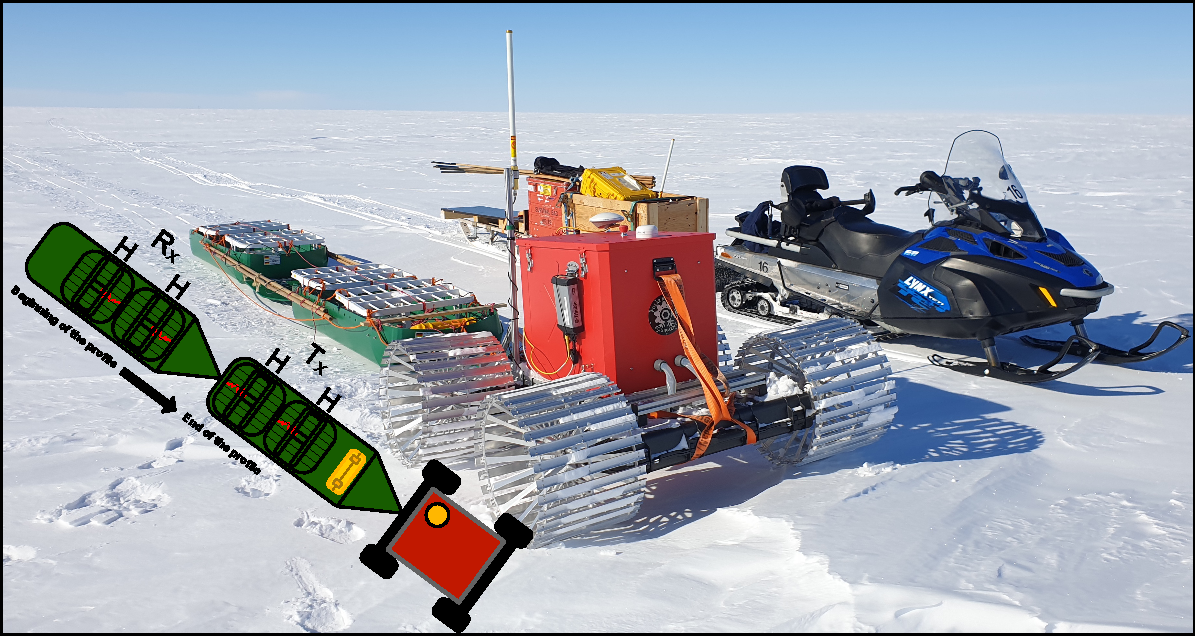
\includegraphics[width=\linewidth]{Figures/MPA_rover.pdf}
	\caption{Pulling the ApRES and sleds using the rover}
	\label{fig_MPA_rover}
\end{figure}
%% ******************************************************
%% ******************************************************
\pagebreak
%% ******************************************************
%% ******************************************************
\section{HF ApRES: Data example, field picture, system setup and profile specifics}
\label{SecHFApRES}
\textbf{JH}
%% ******************************************************
%% ******************************************************
\pagebreak
%% ******************************************************
%% ******************************************************
\section{cApRES: Data example, field picture, system setup and site specifics}
\label{SeccApRES}
\textbf{RE,JH}\\

\textcolor{red}{The cables are not clarified yet. (lengths and colors)}
\begin{figure}[H]
  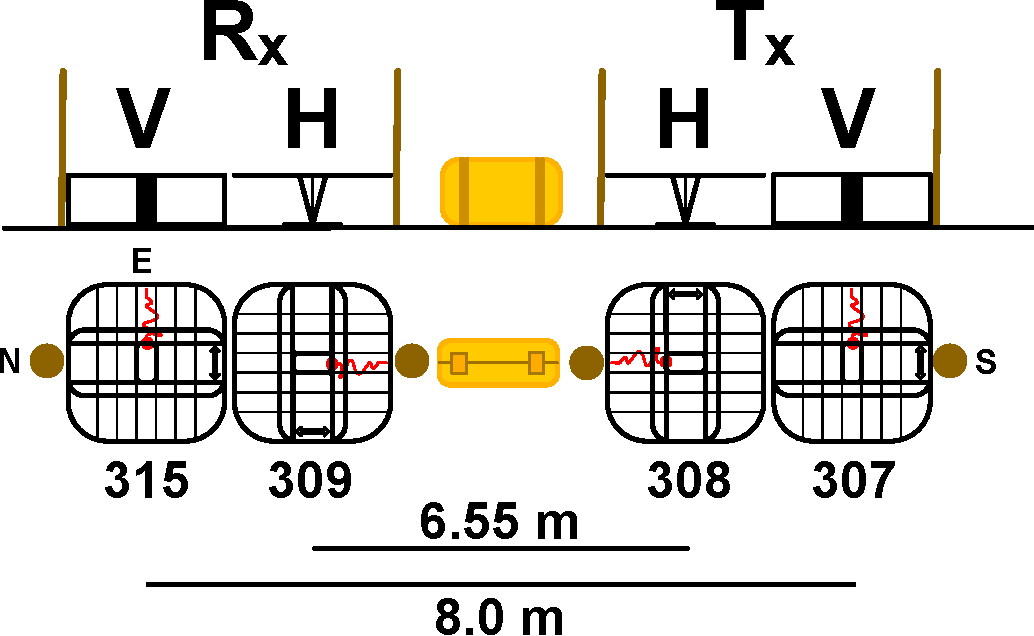
\includegraphics[width=\linewidth]{Figures/cApRES.pdf}
  \caption{cApRES}
  \label{fig_cApRES}
\end{figure}

\begin{table}[H]
  \tiny
  \centering
  \rowcolors{2}{gray!25}{white}
  \begin{tabular}[width=\textwidth]{c c c c c c}
    \rowcolor{gray!50}
    Name & Date & Latitude & Longitude & pRES & Note\\
    \hline
    cApRES & 8\&9.01.2022& S71 36.9565 & W8 25.9803 & 127 & buried\\
    \hline
  \end{tabular}
  \caption{cApRES}
  \label{Table_cApRES}
\end{table}
%% ******************************************************
%% ******************************************************
\pagebreak
%% ******************************************************
%% ******************************************************
\section{Rover-ApRES: Data example, field picture, system setup and site specifics}
\label{SecRoverApRES}
\textbf{This section is written by Reza Ershadi}
(\href{mailto:mohammadreza.ershadi@uni-tuebingen.de}{\color{blue}{Email Me}})\\
\begin{figure}[H]
	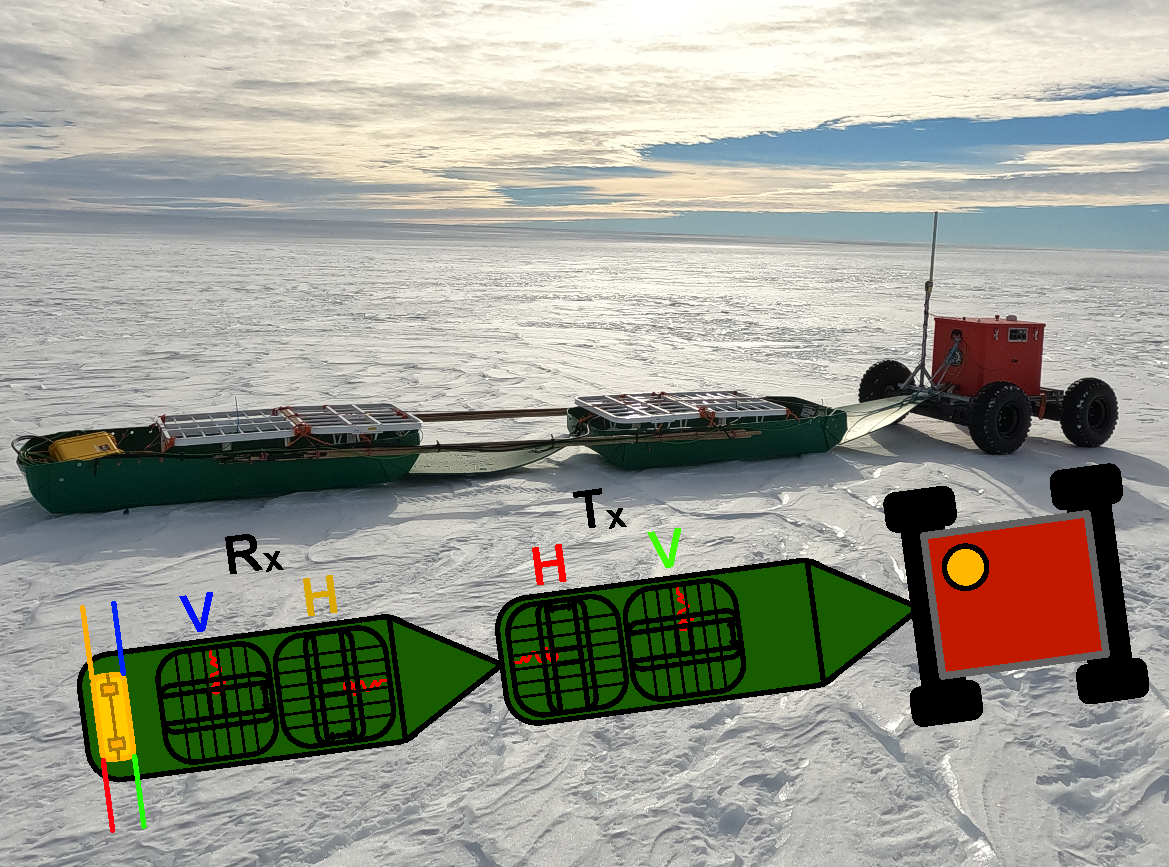
\includegraphics[width=\linewidth]{Figures/Traverse_Rover_Profiling.pdf}
	\caption{Antenna setup for ApRES profiling with the rover and sleds}
	\label{fig_rover}
\end{figure}
\begin{figure}[H]
	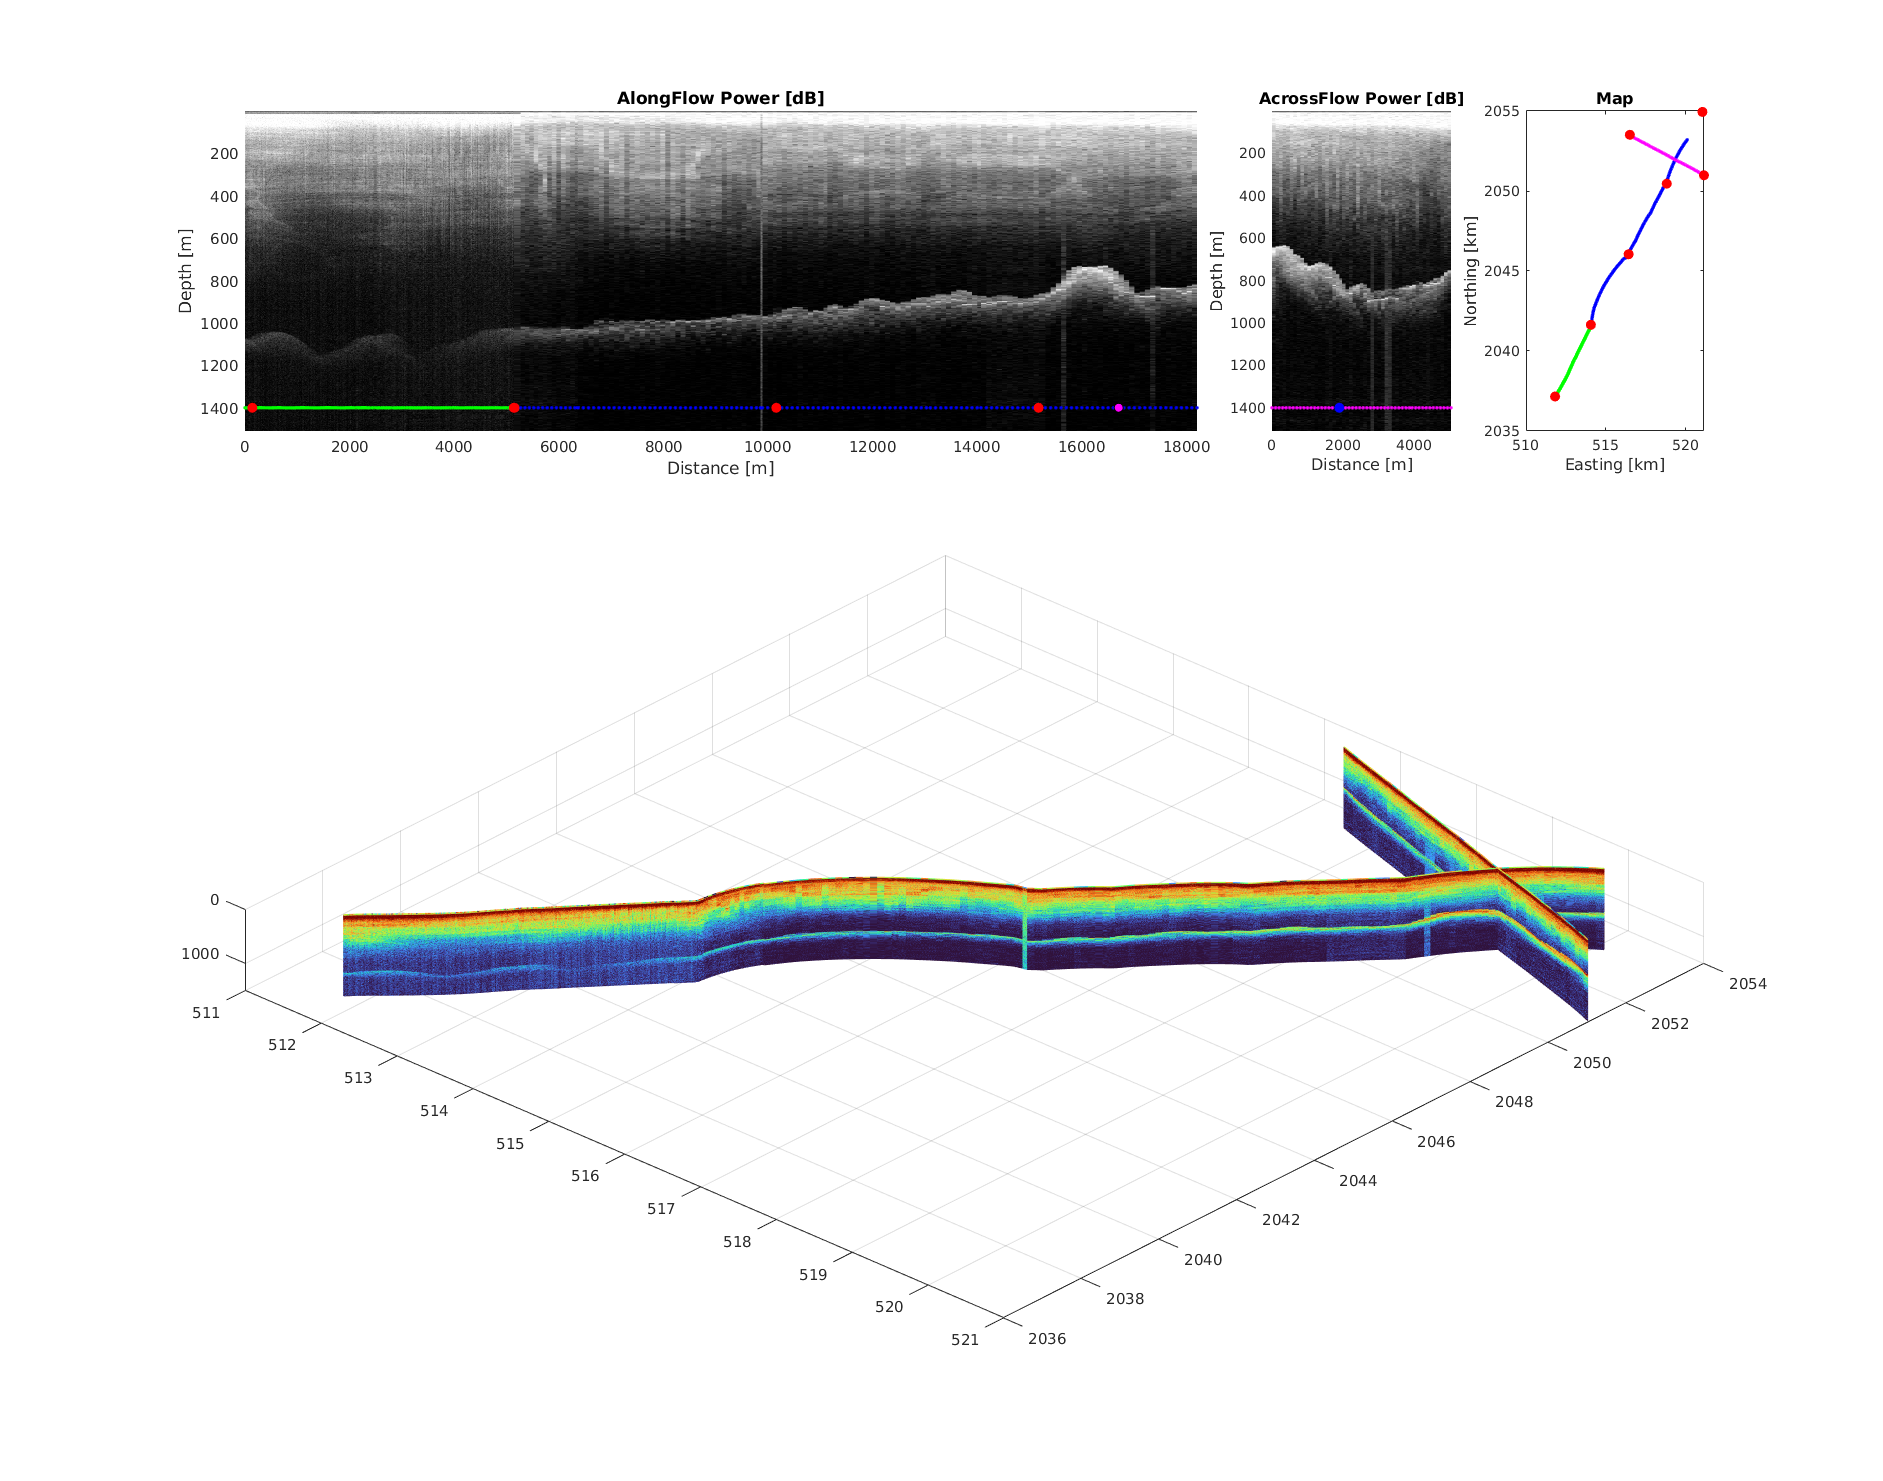
\includegraphics[width=\linewidth]{Figures/Rover_ApRES_Results.png}
	\caption{Radar power obtained by the rover-sled profiling system.}
	\label{fig_rover_res}
\end{figure}

%\ProtocolTable{Setup PulseEkko Radar}{N/A}{PulseEkko 50 MHz}{N/A}{I. Koch}{N/A}

% \begin{minipage}[t]{\textwidth}
%
% \end{minipage}



\end{document}